\section{Instrument Variable EE12.2}
    %\frame{\sectionpage}

%%
\begin{frame}[fragile]{EE12.2}

我們直接從課本的Empirical Exercise 12.2來複習如何用Stata處理內生性問題,並實作2SLS。

\end{frame}

%%
\begin{frame}[fragile]{EE12.2 Questions}
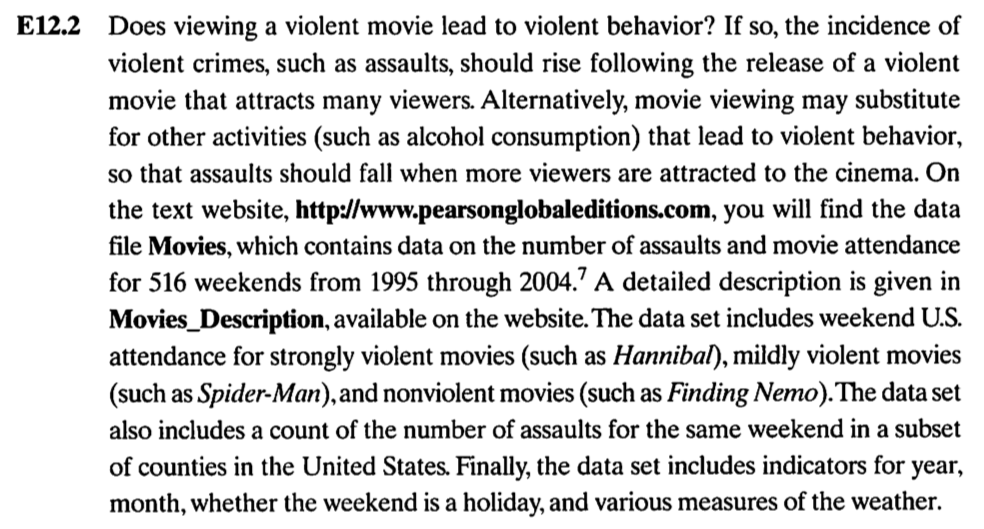
\includegraphics[width=1\textwidth]{Images/EE12-2_1.png}
\end{frame}
%%
\begin{frame}[fragile]{EE12.2 Questions}
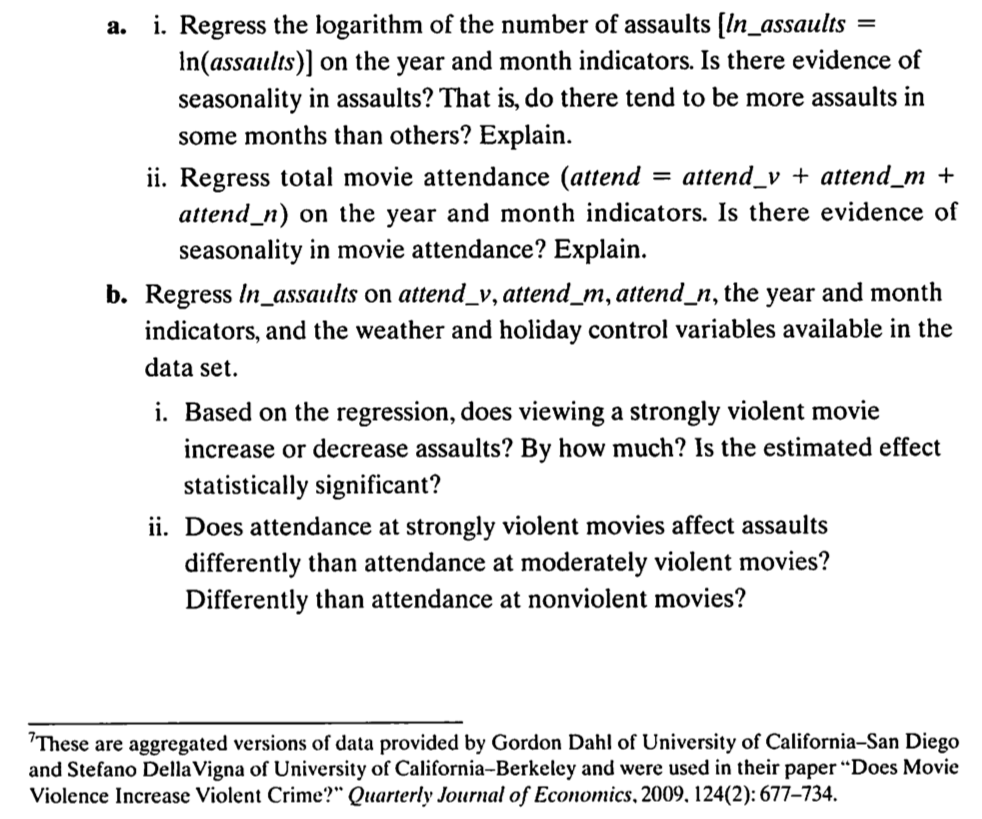
\includegraphics[width=1\textwidth]{Images/EE12-2_2.png}
\end{frame}
%%
\begin{frame}[fragile]{EE12.2 Questions}
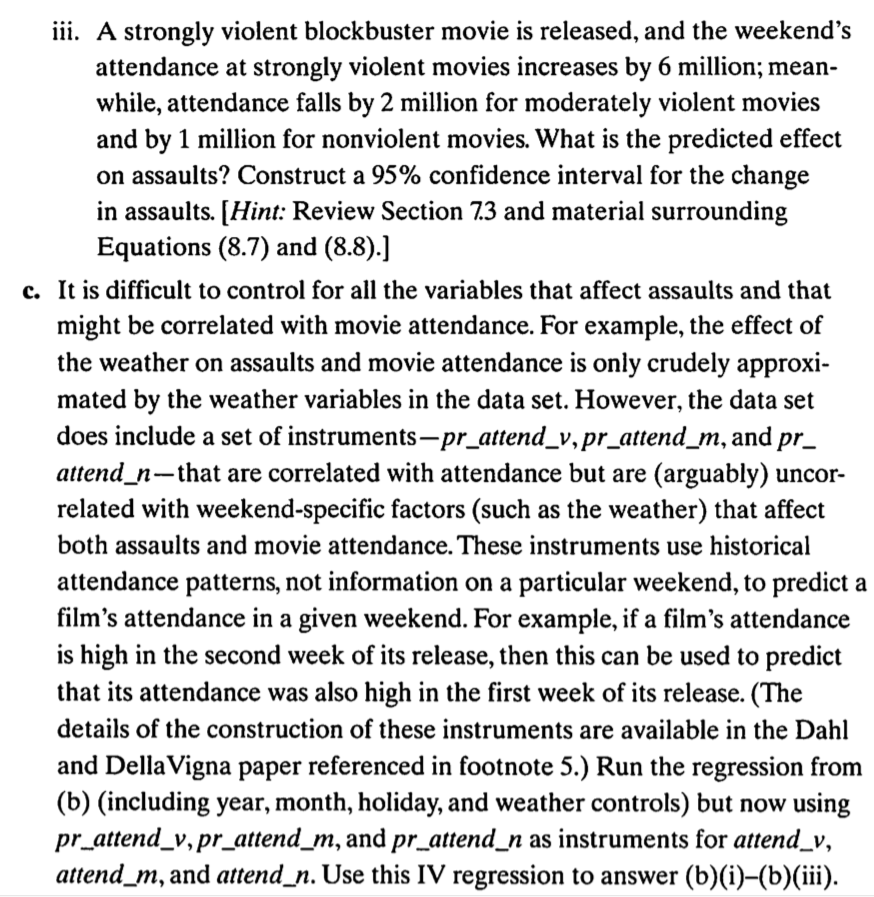
\includegraphics[width=0.6\textwidth]{Images/EE12-2_3.png}
\end{frame}
%%
\begin{frame}[fragile]{EE12.2 Questions}
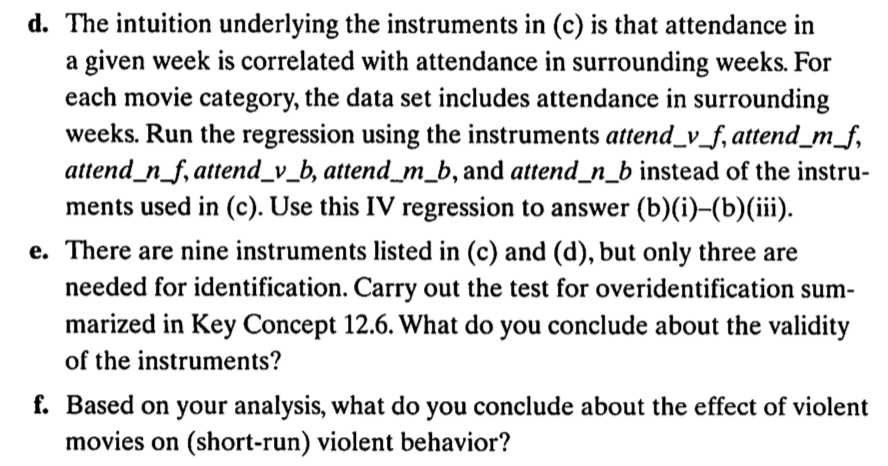
\includegraphics[width=1\textwidth]{Images/EE12-2_4.png}
\end{frame}


%%
\begin{frame}[fragile]{EE12.2 Data Descrptions}

Movie Data

\begin{enumerate}
    \item Observations: 516 weekends
    \item Time Period : 1995-2004
\end{enumerate}
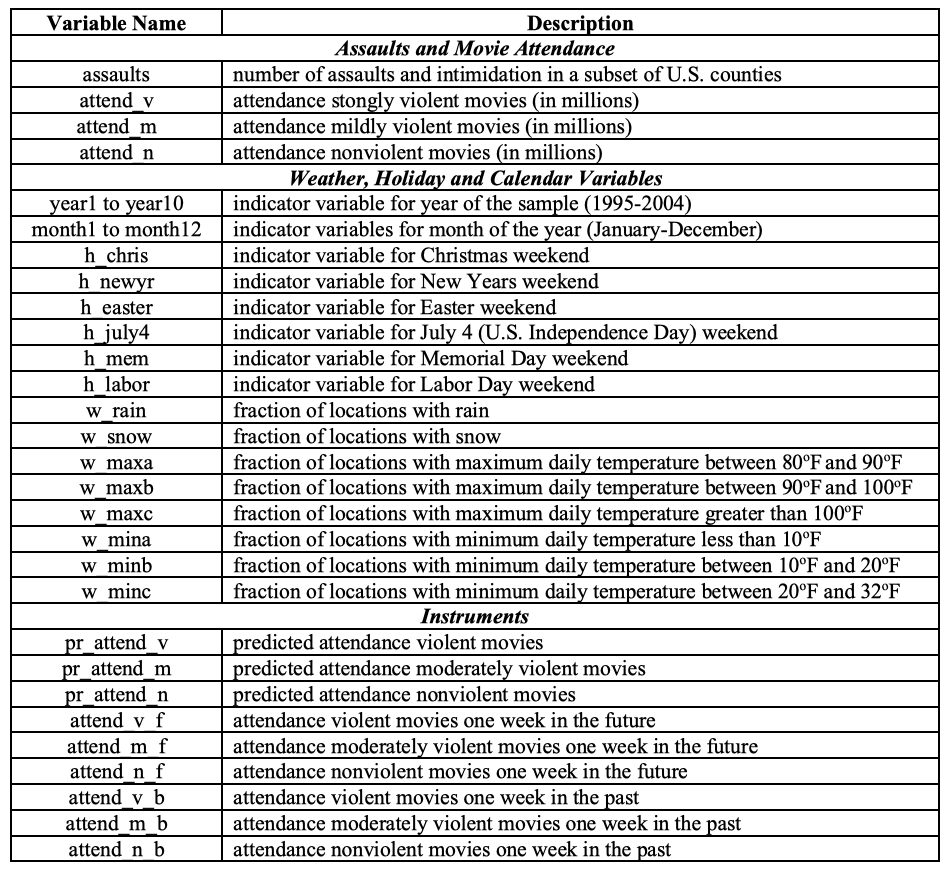
\includegraphics[width=0.6\textwidth]{Images/L4-1_1.png}

\end{frame}


%%
\begin{frame}[fragile]{EE12.2 a(i.)}

To detect whether there is time trend or not:
$$log(assaults) = \beta_0 + \psi_1 year + \psi_2 month + u$$

Or just simply graph a twoway plot with the time indicator.

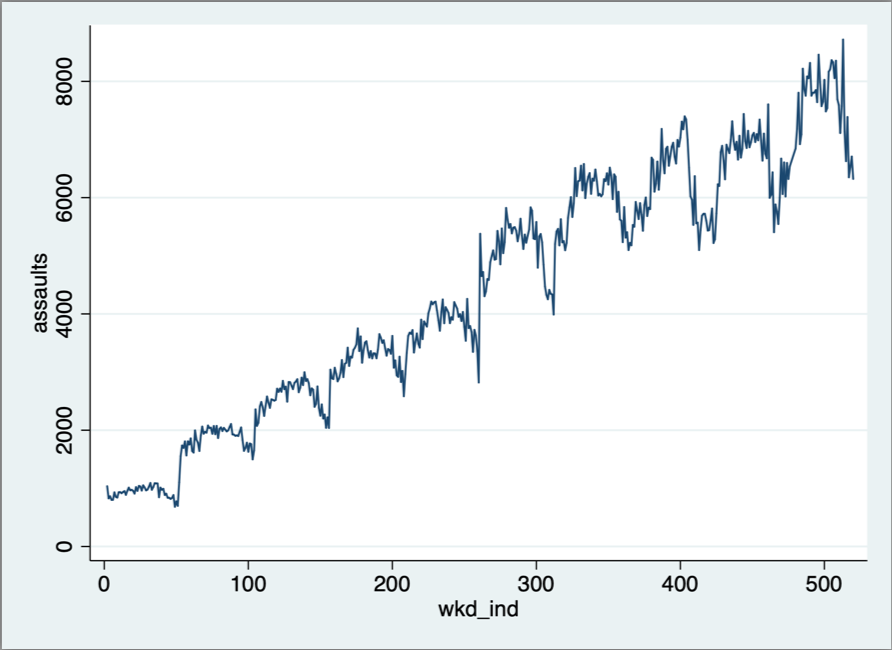
\includegraphics[width=0.8\textwidth]{Images/L4-1_2.png}

\end{frame}


%%
\begin{frame}[fragile]{EE12.2 a(ii.)}

To detect whether there is time trend or not:
$$attendance = \beta_0 + \phi_1 year + \phi_2 month+ \tilde{u}$$

Or just simply graph a twoway plot with the time indicator.

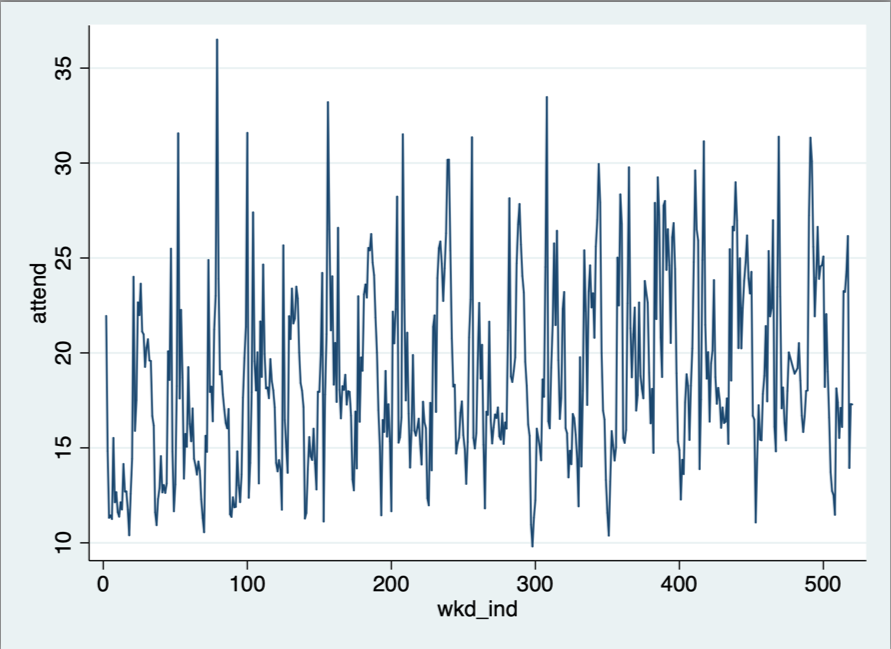
\includegraphics[width=0.8\textwidth]{Images/L4-1_3.png}

\end{frame}


%%
\begin{frame}[fragile]{EE12.2 b}

The original model is:
$$log(assaults) = \beta_0 + \beta_1 attend\textunderscore v +\beta_2 attend\textunderscore m+\beta_3 attend\textunderscore n+ \phi Time+\psi Controls$$

And the variables of interest are \texttt{attend\textunderscore v, attend\textunderscore m, attend\textunderscore n}

Till now, we do not say the variables of interest are exog. or endog.

\end{frame}


%%
\begin{frame}[fragile]{EE12.2 b(iii.)}

The original model is:
$$log(assaults) = \beta_0 + \beta_1 attend\textunderscore v +\beta_2 attend\textunderscore m+\beta_3 attend\textunderscore n+ \phi Time+\psi Controls$$

What we want to know is the change in the dependent variable: $\Delta assaults$.

Let's start from: 
$$\Delta log(assaults) = {\beta_1} \Delta attend\textunderscore v + {\beta_2} \Delta attend\textunderscore m+{\beta_3} \Delta attend\textunderscore n$$

Then,

$$\Delta \widehat{log(assaults)} = \hat{\beta_1} \Delta attend\textunderscore v + \hat{\beta_2} \Delta attend\textunderscore m+\hat{\beta_3} \Delta attend\textunderscore n$$

With the description in the questions:
$$\Delta \widehat{log(assaults)} = 6\hat{\beta_1} - 2 \hat{\beta_2}-\hat{\beta_3}$$

\end{frame}


%%
\begin{frame}[fragile]{EE12.2 b(iii.)}

$$\Delta \widehat{log(assaults)} = 6\hat{\beta_1} - 2 \hat{\beta_2}-\hat{\beta_3}$$

And we can easily calculate the estimate: $\Delta \widehat{log(assaults)} = -.01063206$

That is: $\Delta \widehat{assaults} \approx e^{-.01063206}$

\end{frame}


%%
\begin{frame}[fragile]{EE12.2 b(iii.) conti.}

Given $\Delta \widehat{log(assaults)} = 6\hat{\beta_1} - 2 \hat{\beta_2}-\hat{\beta_3}$

To obtain $se(\Delta \widehat{log(assaults)}) = se(6\hat{\beta_1} - 2 \hat{\beta_2}-\hat{\beta_3})$,

we need to apply approaches in section 7.3.

We may simplify the model by:

$$y =\beta_0 + \beta_1 v+\beta_2 m + \beta_3 n + u$$
Now let's focus on $\beta_1 v+\beta_2 m + \beta_3 n$ only.

Our goal is to have a explanatory variable which has a coefficient equals to the above number.

\end{frame}


%%
\begin{frame}[fragile]{EE12.2 b(iii.) conti.}

Simplified model:

$$y =\beta_0 + \beta_1 v+\beta_2 m + \beta_3 n + u$$

$$y = \beta_1 v+\beta_2 m + \beta_3 n -6\beta_1 n+2\beta_2 n + 6\beta_1 n-2\beta_2 n +u$$

$$y = \beta_1 (v+6n)+\beta_2 (m-2n) + (\beta_3-6\beta_1+2\beta_2) n +u$$

Now we can simply use OLS to obtain the s.e.
\end{frame}

%%
\begin{frame}[fragile]{EE12.2 c}

Now we want to use IVs.

Notations:

$Y: dependent variable$


$X: possibly endog. expanatory variables$

$W: exog. expanatory variables$

$Z: instrument variables$


Recall the 2SLS:

\begin{itemize}
    \item Regress X on Z, W
    \item Obtain $\hat{X}$
    \item Regress Y on $\hat{X}, W$
    \item Obtain the coef. of $\hat{X}$
\end{itemize}

\end{frame}


%%
\begin{frame}[fragile]{EE12.2 c}

Denote

$Y: log(assaults)$

$X: attend\textunderscore v, attend\textunderscore m, attend\textunderscore n$

$W: Time, Holiday, Weather$

$Z: pr\textunderscore attend\textunderscore v, pr\textunderscore attend\textunderscore m, pr\textunderscore attend\textunderscore n$

which are predictions based on historical attendance patterns.

THINK: Why are these variable instruments?

We'll demonstrate the manual 2SLS approach first.

\end{frame}


%%
\begin{frame}[fragile]{EE12.2 c}

We may simply use \texttt{ivreg} or \texttt{ivregress}

The format would be:

\texttt{ivreg Y (X=Z) W, r}

or:

\texttt{ivregress 2sls Y (X=Z) W, r}

\texttt{ivregress gmm Y (X=Z) W, r}

\end{frame}


%%
\begin{frame}[fragile]{EE12.2 d}

Now change the IVs:
$$Z: attend\textunderscore v\textunderscore f, attend\textunderscore m\textunderscore f, attend\textunderscore n\textunderscore f,
\\attend\textunderscore v\textunderscore b, attend\textunderscore m\textunderscore b, attend\textunderscore n\textunderscore b$$

which are the lagged terms and the future terms.

\end{frame}


%%
\begin{frame}[fragile]{EE12.2 e}

For Overidentifying Restriction Test, we first apply J-Test in textbook p.449, then we'll demonstrate a simple and more general command in Stata.

Note that the model now is: 

$Y = \beta X + \gamma W +u$  This is (12.12) in p.438

Denote the residuals obtained in the above regression as $\hat{u}_{2SLS}$.

Then we regress $\hat{u}_{2SLS}$ on $Z, W$, that is:
$$\hat{u}_{2SLS} = \delta Z + \tilde{\gamma} W + e$$
\end{frame}

%%
\begin{frame}[fragile]{EE12.2 e}
And we can obtain the J-statistic from $J=mF$ where

$m = \text{the number of instruments}$

$F = \text{the joint test statistic of } \delta=0}$

$k = \text{the number of exog. variables}$

Under homosk., $J \sim \chi^2(m-k)$
\end{frame}


%%
\begin{frame}[fragile]{EE12.2 e}

An easy command is:

\begin{verbatim}
ivregress Y (X=Z) W, r
estat overid
\end{verbatim}

will give you the test statistic under robust variance covariance estimator.

\end{frame}




